\begin{figure}[t]
\centering
\begin{tabular}{@{}c c c c@{}} % @{} removes padding around the edge of the table
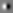
\includegraphics[width=0.2\columnwidth]{\figpath/Gx} &

\includegraphics[width=0.2\columnwidth]{\figpath/Gxx} &
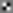
\includegraphics[width=0.2\columnwidth]{\figpath/Gxy} &

\includegraphics[width=0.2\columnwidth]{\figpath/Gxx-Gyy} \\
(a) & (b) & (c) & (d) \\
\noalign{\smallskip}
%
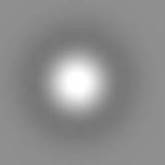
\includegraphics[width=0.2\columnwidth]{\figpath/mono_b} &
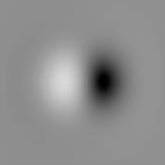
\includegraphics[width=0.2\columnwidth]{\figpath/mono_hx} &

\includegraphics[width=0.2\columnwidth]{\figpath/dt_cwt_r4} &

\includegraphics[width=0.2\columnwidth]{\figpath/dt_cwt_c4} \\
(e) & (f) & (g) & (h) \\
\noalign{\smallskip}
\end{tabular}
%
\caption{(a)~First derivatives $\Gx = \Gy^T$; (b-d)~Second derivatives, $\Gxx = \Gyy^T$, $\Gxy$; and $\Gxx-\Gyy$; (e,f)~Monogenic signal filters $B$ and $h_x = h_y^T$; (g,h)~Real and complex responses of the \dtcwt~ $15^\circ$ subband.}
\label{f:filters}
\end{figure}